\documentclass{article}[18pt]
\usepackage{../../../../format}
\lhead{Networks and Systems - Security}


\begin{document}
\begin{center}
\underline{\huge Identification, authentication, authorization}
\end{center}
\section{Access Control}
Access to the resources:
\begin{itemize}
	\item Claim the identity
	\item Verify the credentials
	\item Check permissions
	\item Grant access
\end{itemize}
\section{Identification}
\textbf{Subject} - An active entity within a system (physical person, script, etc)\\
\textbf{Principal} - An entity that can be granted access (represented by a username, userid, pin etc)\\
\\
The subject identifies itself to the system as a principal
\section{Authentication}
The system verifies the identity of the user\\
\\
\textbf{Object} - Resource that some principals may access or use\\
\\
The system checks that the principal has the permissions to access an object
\section{Credentials}
\begin{itemize}
	\item What do you know? Passwords, PINs
	\item What do you have? Authentication key, passport, ticket, mobile phone
	\item Who you are? Biometrics
\end{itemize}
\section{Passwords}
Common Security Guidelines:
\begin{itemize}
	\item Adopt long passphrases
	\item Avoid easy to guess passwords
	\item Use combination of a-z, A-Z, 0-9 and symbols
	\item Do not write down passwords
	\item Avoid using the same password for multiple services
\end{itemize}
However - when internet users log on to as many as 25 password-protected sites per day, remembering a different and secure password for each one is very difficult.\\
Passwords should be stored in a password manager so you only have to remember one secure password
\section{Authentication Keys}
Authentication keys (e.g. SSH keys)
\begin{itemize}
	\item Similar to passwords, but
	\item RSA-based keys
	\item Subject create private/public key
	\item Share the public key with services
	\item Per device RSA key
\end{itemize}
Advantages:
\begin{itemize}
	\item Public key leak are inconsequential
	\item Compromised device access can be revoked
\end{itemize}
\section{Security Keys}
Authentication keys weakness: Compromised client\\
\\
Solution: Physical security keys:
\begin{itemize}
	\item Static password token (not recommended)
	\item Asynchronous tokens (one-time passwords)
	\item Challenge-response tokens
\end{itemize}
\section{Biometrics}
\textbf{Advantages}:
\begin{itemize}
	\item Non-repudiation: a way to guarantee that an individual who accesses a certain facility cannot later deny using it
\end{itemize}
\textbf{Disadvantages}:
\begin{itemize}
	\item Uncertainty: Compromise between false-positive and false-negatives
\end{itemize}
Receiver Operating Characteristic (ROC) curve
\begin{center}
	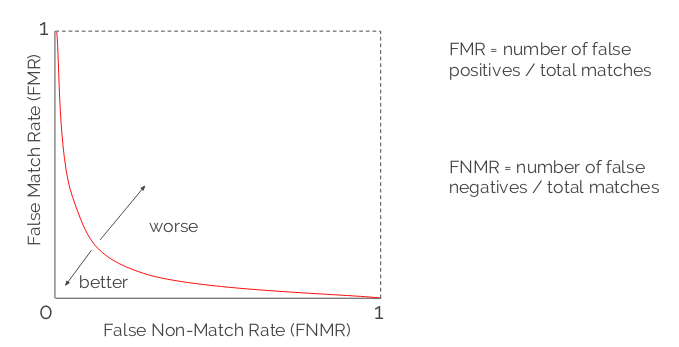
\includegraphics[scale=0.7]{ROC}
\end{center}
Performance policy
\begin{itemize}
	\item Prefer low FMR. E.g. automatic border control. Refer to human on negative result
	\item Prefer now FNMR. E.g. suspect recognition on CCTV. Refer to human on positive result
\end{itemize}
\section{Two-factor authentication}
Two-factor authentication.\\
\\
Combine two authentication factors from:
\begin{itemize}
	\item What you know: password, pin
	\item What you have: mobile phone, authentication key
\end{itemize}
\section{Zero-Knowledge Password Proof}
Objective: Do not reveal anything in the client/server communications about the password.\\
Otherwise we are vulnerable to replay attacks.\\
\\
Most common ZKPP approach: Challenge-response auth:
\begin{itemize}
	\item Serer generate unique challenge value: nonce
	\item Server send nonce to the client
	\item Client computer response = hash(nonce + password)
	\item Client send response back to server
	\item Server compare the response with hash(nonce+stored password)
\end{itemize}

\end{document}